\section{The Chain Rule}
For one variable functions, for instance \( y = f(u) \) and \( u = g(x) \), we
can use the (one-variable) chain rule to compute \(\displaystyle \frac{dy}{dx}
\).
\[ 
  \frac{dy}{dx} = \frac{dy}{du} \frac{du}{dx} \qquad \text{or} \qquad \( y'(x)
  = f'(u)g'(x)\).
\]
An example:
\begin{center}
\fbox{\begin{minipage}{7in}
\begin{example}
  Find \( y'(x) \) where \( y(x) = (x^2 + 1)^5 \)
\end{example}
Let \( u = x^2 + 1 \implies \frac{du}{dx} = 2x \), therefore \( y = u^5 \) and
thus
\[ 
  \frac{dy}{dx} = \frac{dy}{du} \frac{du}{dx} = 5u^4 \cdot (2x) = 10x(x^2
  + 1)^4
\]
\end{minipage}}
\end{center}
\subsection{Chain rule for \( f(x,y) \)}
The chain rule for \( f(x,y) \), for \( x \) and \( y \) being functions of \(
t\) is usually written as
\[ 
  \frac{df}{dt} = \frac{\partial^{}{f}}{\partial{x}^{}} \frac{dx}{dt}
  + \frac{\partial^{}{f}}{\partial{y}^{}} \frac{dy}{dt}
\]
Sometimes \( \displaystyle \frac{\partial^{}{f}}{\partial{x}^{}} \) and \(
\displaystyle \frac{\partial^{}{f}}{\partial{y}^{}} \) are written as \( f_{x}
\) and \( f_{y} \) respectively.
We can derive this equation.
\\\\
Given \( f(x,y) \) with \( x(t) = x \) and \( y(t) = y \),
\[ 
  \frac{df}{dt} = \displaystyle \lim_{\Delta t \to 0} \frac{\Delta f}{\Delta t}
  = \displaystyle \lim_{\Delta t \to 0} \frac{f(x(t+\Delta t), y(t+\Delta t))
  - f(x(t), y(t))}{\Delta t}
\]
Assuming \( f \) is "smooth" and \( \Delta f \) is small, we can make this
following approximation
\[ 
  \Delta f \approx f_x \Delta x + f_y \Delta y
\]
Furthermore
\[ 
  \frac{\Delta f}{\Delta t} \approx f_x \frac{\Delta x}{\Delta t} + f_y
  \frac{\Delta y}{\Delta t}
\]
As \( \Delta t \to 0 \) assuming \( x(t), y(t) \) are smooth, we obtain
\[ 
  \frac{df}{dt} = f_x \frac{dx}{dt} + f_y \frac{dy}{dt}
\]
\begin{note}
You can extrapolate this definition to any number of dimensions. Given
a function \( f(a_1(t), a_2(t), a_3(t) \dots , a_n(t)) \), you can represent its
derivative as
\[ 
  \frac{df}{dt} = \displaystyle \sum_{i=1}^{n}
  \frac{\partial^{}{f}}{\partial{a_i}^{}} \frac{da_i}{dt}
  = \frac{\partial^{}{f}}{\partial{a_1}^{}} \frac{da_1}{dt}
  + \frac{\partial^{}{f}}{\partial{a_2}^{}} \frac{da_2}{dt} + \dots
  + \frac{\partial^{}{f}}{\partial{a_n}^{}} \frac{da_n}{dt}
\]
Where \( n \) is the highest dimension of the function \( f \).
\end{note}

\section{Extended Chain Rules with Tree Diagrams}
For more complex functions, such as \( z = f(u(x(t), y(t)), v(x(t), y(t)) \)
(sub-sub-functions). We can use a tree diagram representation to figure out the
chain rule.
\begin{figure}[h!]
  \centering
  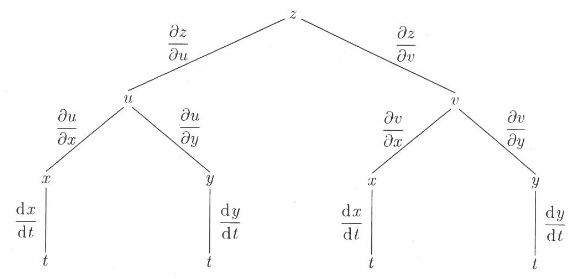
\includegraphics[width=0.6\linewidth]{./lectures/DeepinScreenshot_select-area_20191030114146.png}
\end{figure}

So we have 
\begin{align*}
\frac{dz}{dt} &= 
  \frac{\partial^{}{z}}{\partial{u}^{}}\Big(
    \frac{\partial^{}{u}}{\partial{x}^{}} \frac{dx}{dt}
  + \frac{\partial^{}{u}}{\partial{y}^{}} \frac{dy}{dt}\Big
  ) + \frac{\partial^{}{z}}{\partial{v}^{}}\Big(
    \frac{\partial^{}{v}}{\partial{x}^{}} \frac{dx}{dt}
  + \frac{\partial^{}{v}}{\partial{y}^{}} \frac{dy}{dt}\Big )\\
  &= \Big ( \frac{\partial^{}{z}}{\partial{u}^{}}
    \frac{\partial^{}{u}}{\partial{x}^{}}
    + \frac{\partial^{}{z}}{\partial{v}^{}}
    \frac{\partial^{}{v}}{\partial{x}^{}}\Big ) \frac{dx}{dt} + \Big
    ( \frac{\partial^{}{z}}{\partial{u}^{}}
    \frac{\partial^{}{u}}{\partial{y}^{}}
    + \frac{\partial^{}{z}}{\partial{v}^{}}
  \frac{\partial^{}{v}}{\partial{y}^{}}\Big) \frac{dy}{dt}
\end{align*}

% First 10 mins of the lecture was missed. Update it by watching the lecture
% recording.
%
% TANGENT PLANES

\section{Tangent Planes}
\subsection{Equations for a tangent plane}
Generally for \( z = f(x,y) \) at \( (a,b, f(a,b)) \), we define the
\textbf{tangent plane} to be
\[ 
  z = f(a,b) + f_x(a,b)(x-a) + f_y(a,b)(y-b)
\]
Or
\[ 
  (x,y,z) = (a,b, f(a,b)) + \lambda(1,0, f_x(a,b)) + \mu(0,1, f_y(a,b)),
  \enspace \lambda, \mu \in \mathbb{R} 
\]
Note that \( \lambda = x - a \) and \( \mu = y - b  \) in the latter
expression, you can substitute to check.

\subsection{Directional Derivative}
Define 
$$ f_u (x,y) = \lim_{h \to 0}  \frac{f(x+hu, y+hu_2) - f(x,y)}{h} $$
Where $ ||\underscore{u}||=  1 $. Set $ x = a + hu_1 $, $ y = b + hu_2 $ such that
$ \displaystyle \lim_{h \to 0} (x,y) = (a,b) $ and set $ z(h) = f(x(h), y(h)) $
\par
From the chain rule
$$ \frac{dz}{dh} = \frac{\partial f}{\partial x} \frac{dx}{dh} + \frac{\partial
f}{\partial y} \frac{dy}{dh} $$
$$ = \frac{\partial f}{\partial x} u_1 + \frac{\partial f}{\partial y} u_2 $$
$$ = \Big ( \frac{\partial f}{\partial x}, \frac{\partial f}{\partial y} \Big
  ) \cdot u $$
  \begin{center}
  \fbox{\begin{minipage}{7in}
\begin{example}
    Compute the directional derivative of $ f(x,y) = 4-x^2 - 4y^2 $at (3,-1) in
    the (1,1) direction.
  \begin{align*}
    f(x,y) &= f-x^2 - 4y^2\\
   f_x(x,y) &= -2x \\
   f_y(x,y) &= -8y \\
   f_{(1,1)} (3,-1) &= (f_x(3,-1) , f_y(3,-1)) \cdot \frac{(1,1)}{||(1,1)||} \\
   &= \frac{1}{\sqrt{2}} (-6,8) \cdot (1,1) =  \sqrt{2} 
 \end{align*}
  \end{example}
  \end{minipage}}
  \end{center}
   \subsection{Gradient vector $\nabla f $}
 The gradient vector of $ f $ is a vector with partial derivative compnents 
 $$ \nabla f = (f_x, f_y) = f_x i + f_y j $$
\begin{center}
\fbox{\begin{minipage}{7in}
\begin{example}
 Find the gradient of $ f(x,y) = x^2 - 3(y-1)^2 + 3 $:
\begin{align*}
  \nabla f &= f_x i + f_y j \\
	   &= 2x i - 6(y-1) j
\end{align*}
\end{example}
\end{minipage}}
\end{center}
The gradient $ \nabla f(a,b) $ is perpendicual to the countour line throguh
$ (a,b) $ and in points increasing $ f $. The direction/magnitude of steepest
slope at $ (a,b) $ are given by $ \nabla f(a,b) $ and $ ||\nabla f(a,b)|| $. We can understand these two facts by
